% !TEX root = ../main.tex
\chapter{Ensemble Methods}
\label{ch:ensembles}

\begin{intuition}[title=\textbf{Why Combine Models?}]
A single decision tree is a high-variance estimator: small perturbations of the training set can lead to radically different trees. By aggregating many such estimators, we can dramatically reduce variance while preserving (or even improving) predictive accuracy. This chapter formalises that intuition and develops the two great families of ensembles: \emph{bagging} and \emph{boosting}.
\end{intuition}

%% ----------------------------------------------------------------
\section{Bias--Variance Decomposition for Ensembles}

\begin{theorem}[Variance Reduction by Averaging]
Let $f_1,\dots,f_B$ be $B$ estimators, each with $\E[f_b(\bm{x})]=\mu(\bm{x})$, $\Var[f_b(\bm{x})]=\sigma^2$, and pairwise correlation $\rho$. Define the ensemble prediction
\[
  \bar{f}(\bm{x}) = \frac{1}{B}\sum_{b=1}^{B} f_b(\bm{x}).
\]
Then
\[
  \Var[\bar{f}(\bm{x})] = \rho\,\sigma^2 + \frac{1-\rho}{B}\,\sigma^2.
\]
\end{theorem}

\begin{proof}
\[
  \Var\!\Bigl[\frac{1}{B}\sum_b f_b\Bigr]
  = \frac{1}{B^2}\Bigl[\sum_b \Var[f_b] + \sum_{b\neq b'}\Cov(f_b,f_{b'})\Bigr]
  = \frac{1}{B^2}\bigl[B\sigma^2 + B(B-1)\rho\sigma^2\bigr]
  = \rho\sigma^2 + \frac{1-\rho}{B}\sigma^2. \qedhere
\]
\end{proof}

\begin{remark}
As $B\to\infty$, $\Var[\bar f]\to\rho\sigma^2$. The irreducible term $\rho\sigma^2$ vanishes only if the base learners are uncorrelated ($\rho=0$). Bagging and random forests are precisely designed to reduce $\rho$.
\end{remark}

%% ----------------------------------------------------------------
\section{Bagging (Bootstrap Aggregating)}

\begin{definition}[Bootstrap Sample]
Given a dataset $\mathcal{D}=\{(\bm{x}_i,y_i)\}_{i=1}^n$, a \emph{bootstrap sample} $\mathcal{D}^{*b}$ is obtained by drawing $n$ observations uniformly with replacement from $\mathcal{D}$.
\end{definition}

\begin{algorithme}[title=\textbf{Bagging}]
\begin{enumerate}
  \item For $b=1,\dots,B$:
    \begin{enumerate}
      \item Draw bootstrap sample $\mathcal{D}^{*b}$ from $\mathcal{D}$.
      \item Fit base learner $\hat f_b$ on $\mathcal{D}^{*b}$.
    \end{enumerate}
  \item Aggregate:
    \[
      \hat f_{\text{bag}}(\bm{x}) =
      \begin{cases}
        \frac{1}{B}\sum_{b=1}^B \hat f_b(\bm{x}) & \text{(regression)},\\[4pt]
        \argmax_k \sum_{b=1}^B \ind\{\hat f_b(\bm{x})=k\} & \text{(classification)}.
      \end{cases}
    \]
\end{enumerate}
\end{algorithme}

\begin{proposition}[Out-of-Bag Probability]
The probability that observation $i$ is \emph{not} selected in a particular bootstrap sample is
\[
  \Bigl(1-\frac{1}{n}\Bigr)^n \xrightarrow{n\to\infty} e^{-1}\approx 0.368.
\]
Hence roughly 36.8\% of observations are left out of each bootstrap sample.
\end{proposition}

%% ----------------------------------------------------------------
\section{Random Forests}

\begin{definition}[Random Forest]
A \emph{random forest} is a bagged ensemble of decision trees where, at each split, only a random subset of $m$ features (out of $p$) is considered as candidates. Typical defaults are $m=\lfloor\sqrt{p}\rfloor$ (classification) and $m=\lfloor p/3\rfloor$ (regression).
\end{definition}

The feature subsampling further decorrelates the trees, reducing $\rho$ in the variance formula and hence reducing overall variance.

\subsection{Out-of-Bag Error}

\begin{definition}[OOB Error]
For each observation $(\bm{x}_i,y_i)$, the \emph{OOB prediction} is the aggregate prediction using only those trees $b$ for which $i\notin\mathcal{D}^{*b}$:
\[
  \hat f_{\text{OOB}}(\bm{x}_i) = \frac{1}{|\{b:i\notin\mathcal{D}^{*b}\}|}
    \sum_{b:\,i\notin\mathcal{D}^{*b}} \hat f_b(\bm{x}_i).
\]
The OOB error is the average loss over all training observations evaluated via their OOB predictions. It provides an unbiased estimate of generalisation error without a separate validation set.
\end{definition}

\begin{figure}[ht]
\centering
\begin{tikzpicture}[
    tree/.style={isosceles triangle, draw, shape border rotate=90,
      minimum height=1.4cm, minimum width=1cm, fill=blue!10},
    data/.style={rectangle, draw, minimum width=2cm, minimum height=0.5cm, fill=gray!15}
  ]
  \node[data] (D) at (0,0) {$\mathcal{D}$};
  \foreach \i in {1,2,3,4}{
    \node[data] (B\i) at (-3+2*\i, -1.5) {$\mathcal{D}^{*\i}$};
    \draw[-stealth] (D) -- (B\i) node[midway,right,font=\scriptsize]{bootstrap};
    \node[tree] (T\i) at (-3+2*\i, -3.5) {};
    \draw[-stealth] (B\i) -- (T\i);
  }
  \node[rectangle, draw, rounded corners, fill=green!10, minimum width=2.5cm] (agg) at (2, -5.5) {Majority Vote / Average};
  \foreach \i in {1,2,3,4}{
    \draw[-stealth] (T\i.south) -- (agg);
  }
\end{tikzpicture}
\caption{Schematic of the bagging / random forest procedure.}
\label{fig:bagging-schema}
\end{figure}

%% ----------------------------------------------------------------
\section{AdaBoost}

Boosting builds the ensemble \emph{sequentially}: each new learner focuses on the examples that previous learners misclassified.

\begin{algorithme}[title=\textbf{AdaBoost (Binary Classification)}]
\textbf{Input:} Training set $\{(\bm{x}_i,y_i)\}_{i=1}^n$, $y_i\in\{-1,+1\}$; number of rounds $T$.\\[4pt]
Initialise weights $w_i^{(1)}=1/n$ for all $i$.\\[2pt]
For $t=1,\dots,T$:
\begin{enumerate}
  \item Fit weak learner $h_t$ to training data weighted by $\bm{w}^{(t)}$.
  \item Compute weighted error:
    $\epsilon_t = \sum_{i=1}^n w_i^{(t)}\,\ind\{h_t(\bm{x}_i)\neq y_i\}.$
  \item Compute learner weight:
    $\alpha_t = \tfrac{1}{2}\ln\!\bigl(\frac{1-\epsilon_t}{\epsilon_t}\bigr).$
  \item Update sample weights:
    $w_i^{(t+1)} = \frac{w_i^{(t)}\exp(-\alpha_t\, y_i\, h_t(\bm{x}_i))}{Z_t},$
    where $Z_t$ is a normalisation constant.
\end{enumerate}
\textbf{Output:} $H(\bm{x})=\operatorname{sign}\!\bigl(\sum_{t=1}^T \alpha_t\, h_t(\bm{x})\bigr).$
\end{algorithme}

\begin{theorem}[AdaBoost Training Error Bound]
The training error of the final classifier satisfies
\[
  \frac{1}{n}\sum_{i=1}^n \ind\{H(\bm{x}_i)\neq y_i\}
  \;\leq\; \prod_{t=1}^T Z_t
  \;=\; \prod_{t=1}^T 2\sqrt{\epsilon_t(1-\epsilon_t)}.
\]
\end{theorem}

\begin{proof}
For any misclassified example, $y_i H(\bm{x}_i)<0$, so $\ind\{H(\bm{x}_i)\neq y_i\}\leq \exp(-y_i\sum_t\alpha_t h_t(\bm{x}_i))$. Averaging over $i$ and unrolling the weight updates gives
\[
  \frac{1}{n}\sum_i \exp\!\Bigl(-y_i\sum_t \alpha_t h_t(\bm{x}_i)\Bigr)
  = \prod_{t=1}^T Z_t.
\]
Each normalisation constant equals $Z_t = 2\sqrt{\epsilon_t(1-\epsilon_t)}$, which follows by direct computation of the partition function using the definition of $\alpha_t$.
\end{proof}

\begin{remark}
The choice $\alpha_t=\frac{1}{2}\ln\frac{1-\epsilon_t}{\epsilon_t}$ is exactly the value that minimises $Z_t$ (and hence the training error upper bound) at each round. This is derived by differentiating $Z_t$ with respect to $\alpha_t$ and setting the derivative to zero.
\end{remark}

%% ----------------------------------------------------------------
\section{Gradient Boosting}

\begin{definition}[Gradient Boosting]
Gradient boosting builds an additive model $F_T(\bm{x})=\sum_{t=1}^T \gamma_t h_t(\bm{x})$ by performing \emph{functional gradient descent} in the space of functions. At round $t$, the pseudo-residuals are
\[
  r_i^{(t)} = -\frac{\partial \mathcal{L}(y_i, F(\bm{x}_i))}{\partial F(\bm{x}_i)}\bigg|_{F=F_{t-1}},
\]
and the next base learner $h_t$ is fitted to $({\bm{x}_i, r_i^{(t)}})_{i=1}^n$.
\end{definition}

For squared loss $\mathcal{L}(y,F)=\frac{1}{2}(y-F)^2$, the pseudo-residuals are simply $r_i^{(t)}=y_i - F_{t-1}(\bm{x}_i)$, i.e.\ the actual residuals.

\subsection{XGBoost and LightGBM}

\begin{keyformulas}[title=\textbf{XGBoost Objective}]
At round $t$, XGBoost minimises a second-order approximation of the regularised objective:
\[
  \tilde{\mathcal{L}}^{(t)} = \sum_{i=1}^n \bigl[g_i\, h_t(\bm{x}_i) + \tfrac{1}{2}h_i\, h_t(\bm{x}_i)^2\bigr]
  + \Omega(h_t),
\]
where $g_i=\partial_{F}\mathcal{L}(y_i,F_{t-1}(\bm{x}_i))$, $\;h_i=\partial_{F}^2\mathcal{L}(y_i,F_{t-1}(\bm{x}_i))$, and $\Omega(h)=\gamma\, T_{\text{leaves}} + \frac{\lambda}{2}\sum_j w_j^2$ is a regularisation term penalising tree complexity.

The optimal leaf weight for leaf $j$ is:
\[
  w_j^* = -\frac{\sum_{i\in I_j} g_i}{\sum_{i\in I_j} h_i + \lambda},
\]
and the corresponding gain for a candidate split is:
\[
  \text{Gain} = \frac{1}{2}\Biggl[\frac{(\sum_{i\in I_L}g_i)^2}{\sum_{i\in I_L}h_i+\lambda}
  + \frac{(\sum_{i\in I_R}g_i)^2}{\sum_{i\in I_R}h_i+\lambda}
  - \frac{(\sum_{i\in I_j}g_i)^2}{\sum_{i\in I_j}h_i+\lambda}\Biggr] - \gamma.
\]
\end{keyformulas}

\begin{bestpractice}[title=\textbf{XGBoost vs LightGBM}]
\begin{itemize}
  \item \textbf{XGBoost}: level-wise tree growth; exact or approximate split finding via quantile sketch.
  \item \textbf{LightGBM}: leaf-wise growth (best-first); Gradient-based One-Side Sampling (GOSS) and Exclusive Feature Bundling (EFB) for speed on large datasets.
  \item Both support GPU training, early stopping, and built-in cross-validation.
\end{itemize}
\end{bestpractice}

%% ----------------------------------------------------------------
\section{Bagging vs Boosting: A Visual Comparison}

\begin{figure}[ht]
\centering
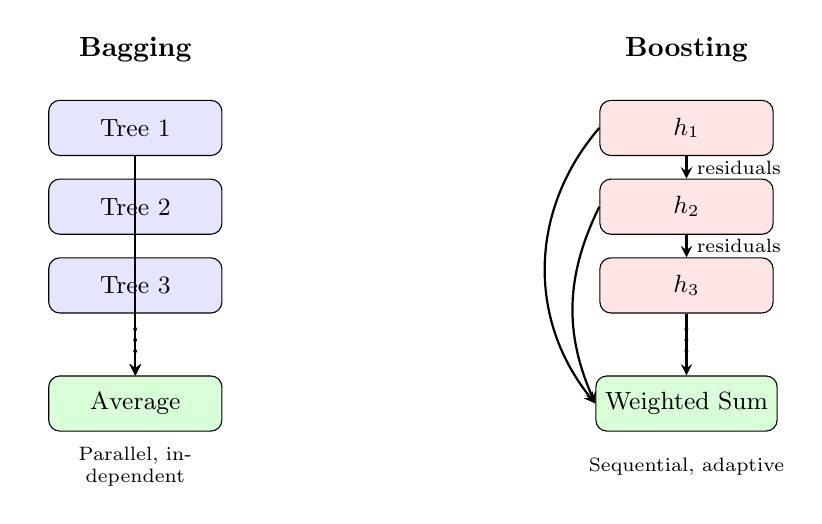
\begin{tikzpicture}[
    box/.style={rectangle, draw, rounded corners, minimum width=2.2cm,
      minimum height=0.7cm, font=\small},
    arr/.style={-stealth, thick}
  ]
  % Bagging side
  \node[font=\bfseries] at (-3.5, 3) {Bagging};
  \node[box, fill=blue!10] (b1) at (-3.5, 2) {Tree 1};
  \node[box, fill=blue!10] (b2) at (-3.5, 1) {Tree 2};
  \node[box, fill=blue!10] (b3) at (-3.5, 0) {Tree 3};
  \node[font=\Large] at (-3.5, -0.6) {$\vdots$};
  \node[box, fill=green!15] (ba) at (-3.5, -1.5) {Average};
  \draw[arr] (b1) -- (ba);
  \draw[arr] (b2) -- (ba);
  \draw[arr] (b3) -- (ba);
  \node[font=\scriptsize, text width=2.5cm, align=center] at (-3.5, -2.3) {Parallel, independent};

  % Boosting side
  \node[font=\bfseries] at (3.5, 3) {Boosting};
  \node[box, fill=red!10] (h1) at (3.5, 2) {$h_1$};
  \node[box, fill=red!10] (h2) at (3.5, 1) {$h_2$};
  \node[box, fill=red!10] (h3) at (3.5, 0) {$h_3$};
  \node[font=\Large] at (3.5, -0.6) {$\vdots$};
  \node[box, fill=green!15] (bo) at (3.5, -1.5) {Weighted Sum};
  \draw[arr] (h1) -- (h2) node[midway, right, font=\scriptsize]{residuals};
  \draw[arr] (h2) -- (h3) node[midway, right, font=\scriptsize]{residuals};
  \draw[arr] (h1.west) to[bend right=40] (bo.west);
  \draw[arr] (h2.west) to[bend right=25] (bo.west);
  \draw[arr] (h3) -- (bo);
  \node[font=\scriptsize, text width=2.5cm, align=center] at (3.5, -2.3) {Sequential, adaptive};
\end{tikzpicture}
\caption{Bagging (parallel, reduces variance) vs Boosting (sequential, reduces bias).}
\label{fig:bag-vs-boost}
\end{figure}

%% ----------------------------------------------------------------
\section{Comparison of Ensemble Methods}

\begin{table}[ht]
\centering
\caption{Summary of ensemble methods.}
\label{tab:ensemble-comparison}
\begin{tabular}{lcccc}
\toprule
\textbf{Method} & \textbf{Strategy} & \textbf{Main effect} & \textbf{Base learner} & \textbf{Risk} \\
\midrule
Bagging        & Parallel  & $\downarrow$ Variance & Any (often trees) & Low overfitting \\
Random Forest  & Parallel  & $\downarrow\downarrow$ Variance & Decorrelated trees & Low overfitting \\
AdaBoost       & Sequential & $\downarrow$ Bias     & Weak (stumps)     & Sensitive to noise \\
Gradient Boost & Sequential & $\downarrow$ Bias     & Regression trees  & Can overfit \\
XGBoost        & Sequential & $\downarrow$ Bias     & Regularised trees & Robust \\
\bottomrule
\end{tabular}
\end{table}

%% ----------------------------------------------------------------
\section{Implementation in Python}

\begin{codeblock}[title=\textbf{Random Forest, AdaBoost, and Gradient Boosting with scikit-learn}]
\begin{minted}{python}
import numpy as np
from sklearn.datasets import make_classification
from sklearn.model_selection import cross_val_score
from sklearn.ensemble import (
    BaggingClassifier,
    RandomForestClassifier,
    AdaBoostClassifier,
    GradientBoostingClassifier,
)
from sklearn.tree import DecisionTreeClassifier

# Generate synthetic data
X, y = make_classification(
    n_samples=1000, n_features=20,
    n_informative=10, random_state=42
)

models = {
    "Bagging (Trees)": BaggingClassifier(
        estimator=DecisionTreeClassifier(),
        n_estimators=100, random_state=42
    ),
    "Random Forest": RandomForestClassifier(
        n_estimators=100, max_features="sqrt", random_state=42
    ),
    "AdaBoost": AdaBoostClassifier(
        n_estimators=100, learning_rate=0.5, random_state=42
    ),
    "Gradient Boosting": GradientBoostingClassifier(
        n_estimators=200, learning_rate=0.1,
        max_depth=3, random_state=42
    ),
}

for name, model in models.items():
    scores = cross_val_score(model, X, y, cv=5, scoring="accuracy")
    print(f"{name:25s}  accuracy = {scores.mean():.4f} +/- {scores.std():.4f}")
\end{minted}
\end{codeblock}

\begin{codeoutput}
\begin{verbatim}
Bagging (Trees)            accuracy = 0.9190 +/- 0.0222
Random Forest              accuracy = 0.9320 +/- 0.0198
AdaBoost                   accuracy = 0.9090 +/- 0.0265
Gradient Boosting          accuracy = 0.9410 +/- 0.0177
\end{verbatim}
\end{codeoutput}

\begin{codeblock}[title=\textbf{OOB Error and Feature Importance}]
\begin{minted}{python}
# OOB error estimation (no separate validation set needed)
rf = RandomForestClassifier(
    n_estimators=300, oob_score=True, random_state=42
)
rf.fit(X, y)
print(f"OOB accuracy: {rf.oob_score_:.4f}")

# Feature importances (mean decrease in impurity)
importances = rf.feature_importances_
indices = np.argsort(importances)[::-1]
print("\nTop 5 features:")
for rank, idx in enumerate(indices[:5], 1):
    print(f"  {rank}. Feature {idx}: importance = {importances[idx]:.4f}")
\end{minted}
\end{codeblock}

\begin{codeblock}[title=\textbf{XGBoost with Early Stopping}]
\begin{minted}{python}
from sklearn.model_selection import train_test_split
from xgboost import XGBClassifier

X_train, X_test, y_train, y_test = train_test_split(
    X, y, test_size=0.2, random_state=42
)

xgb = XGBClassifier(
    n_estimators=500, learning_rate=0.05,
    max_depth=4, reg_lambda=1.0, subsample=0.8,
    colsample_bytree=0.8, early_stopping_rounds=20,
    eval_metric="logloss", random_state=42
)
xgb.fit(
    X_train, y_train,
    eval_set=[(X_test, y_test)], verbose=False
)
print(f"Best iteration: {xgb.best_iteration}")
print(f"Test accuracy:  {xgb.score(X_test, y_test):.4f}")
\end{minted}
\end{codeblock}

%% ----------------------------------------------------------------
\section{Exercises}

\begin{exercise}[Variance of Bagged Estimator]
Let $f_1,\dots,f_B$ be i.i.d.\ with variance $\sigma^2$. Show that the variance of their average is $\sigma^2/B$. Now suppose they share pairwise correlation $\rho>0$; prove the formula $\Var[\bar f]=\rho\sigma^2+(1-\rho)\sigma^2/B$ and interpret the limit as $B\to\infty$.
\end{exercise}

\begin{exercise}[AdaBoost Weight Update]
Show that the choice $\alpha_t=\frac{1}{2}\ln\frac{1-\epsilon_t}{\epsilon_t}$ minimises the normalisation constant $Z_t=\sum_i w_i^{(t)}\exp(-\alpha_t y_i h_t(\bm{x}_i))$. \emph{Hint:} Split the sum into correctly and incorrectly classified subsets.
\end{exercise}

\begin{exercise}[Random Forest vs Bagging]
Using the \texttt{make\_classification} dataset above with $p=50$ features, compare the 5-fold CV accuracy of \texttt{BaggingClassifier} (full trees) and \texttt{RandomForestClassifier} for $B\in\{10,50,100,200,500\}$. Plot both curves. At what $B$ does each method plateau?
\end{exercise}

\begin{exercise}[Gradient Boosting from Scratch]
Implement gradient boosting for regression (squared loss) using \texttt{DecisionTreeRegressor(max\_depth=3)} as the base learner. Use a learning rate $\eta=0.1$ and $T=100$ rounds. Compare your implementation with \texttt{GradientBoostingRegressor} on the Boston-style housing dataset.
\end{exercise}

\begin{exercise}[Hyperparameter Tuning for XGBoost]
Use \texttt{RandomizedSearchCV} to tune the following XGBoost hyperparameters on a dataset of your choice: \texttt{max\_depth} $\in\{3,\dots,10\}$, \texttt{learning\_rate} $\in[0.01,0.3]$, \texttt{subsample} $\in[0.6,1.0]$, \texttt{colsample\_bytree} $\in[0.6,1.0]$, \texttt{n\_estimators} $\in\{100,\dots,1000\}$. Report the best parameters and test set performance.
\end{exercise}
